\documentclass[11pt]{article}
\usepackage[margin=1in]{geometry}
\usepackage{amsmath,amssymb}
\usepackage[T1]{fontenc}
\usepackage[utf8]{inputenc}
\usepackage{parskip}
\usepackage{graphicx}
\usepackage{alltt}
\usepackage{url}
\DeclareMathOperator*{\argmin}{arg\,min}
\DeclareMathOperator*{\argmax}{arg\,max}
\newcommand{\slide}[2]{\subsection*{Slide #1: #2}}
\newcommand{\poll}[1]{\begin{center}\fbox{\parbox{0.85\textwidth}{\centering \textbf{Slido poll} \\ #1}}\end{center}}
\setlength{\parindent}{0pt}

\title{Algorithms COMP.5030 --- Intro Lecture\\[1ex]\large (structured from NuMarkdown-8B-Thinking OCR, corrected)}
\author{Prof.\ Hugo A.\ Akitaya}
\date{}

\begin{document}
\maketitle

\section{Course Introduction}

\slide{1}{Title}
\begin{center}
\textbf{\Large Algorithms COMP.5030}\\[1ex]
Prof.\ Hugo A.\ Akitaya
\end{center}

\slide{2}{What is Computer Science?}
Map of Computer Science infographic.
\begin{center}
\urlstyle{tt}\url{https://www.youtube.com/watch?v=SzJ46YA_RaA}
\end{center}

\slide{3}{Why study algorithms?}
\begin{itemize}
  \item Job interviews.
  \item Solving (new/old) problems.
  \item Being a better coder.
  \item Understanding what can or cannot be done, and why.
\end{itemize}
(Image: ``It's dangerous to go alone! Take this.'' --- \textit{The Legend of Zelda}.)

\slide{4}{Algorithms?}
Comic panels illustrating the struggle with algorithms (xkcd).
\begin{center}
\url{https://xkcd.com/1831/}
\end{center}

\slide{5}{Prerequisites}
\begin{itemize}
  \item Discrete Math:
  \begin{itemize}
    \item Proof techniques
    \item Basic graph theory
  \end{itemize}
  \item COMP.4040:
  \begin{itemize}
    \item Fundamental algorithms
    \item Asymptotic analysis
    \item Basic data types/structures
    \item Writing pseudocode
  \end{itemize}
\end{itemize}
(Image: cover of \textit{Introduction to Algorithms} by Cormen et al.)

\slide{6}{Blackboard}
\begin{itemize}
  \item Syllabus
  \item Homework
  \item Attendance
  \item Slido
\end{itemize}

\slide{7}{Poll: Why 5030?}
\poll{Why 5030? (open-ended question)}

\section{Review: The Maximum-Profit Problem}

\slide{8}{Problem statement (CLRS 4.1)}
\textbf{Problem:} You are allowed to buy and sell a stock exactly once. You know the future and have a graph of future stock prices. \textbf{Maximize your profit.}

\begin{center}
\begin{tabular}{|c||*{17}{c|}}
\hline
Day & 0 & 1 & 2 & 3 & 4 & 5 & 6 & 7 & 8 & 9 & 10 & 11 & 12 & 13 & 14 & 15 & 16\\\hline
Price & 100 & 113 & 110 & 85 & 105 & 102 & 86 & 63 & 81 & 101 & 94 & 106 & 101 & 79 & 94 & 90 & 97\\\hline
\end{tabular}
\end{center}

\slide{9}{Understanding the problem}
\begin{itemize}
  \item \textbf{Input:} Array of integers $A[1..n]$.
  \item \textbf{Output:} Indices $i$ and $j$ (with $i \le j$) such that $A[j] - A[i]$ is maximized.
\end{itemize}
(Line graph of the daily prices from Slide~8.)

\slide{10}{Poll: What is the optimal solution?}
\poll{What is the optimal solution? (multiple choice)}

\slide{11}{Poll: Which of these solutions is better?}
\poll{Which of these solutions is better? (multiple choice)}

\slide{12}{A little more math}
Profit function:
\[
  p : \{(i,j) \mid i,j \in [0..n-1],\ i \le j\} \to \mathbb{R},
  \qquad p(i,j) = A[j] - A[i].
\]
\begin{itemize}
  \item $p(1,3) = ?$
  \item Optimal solution: $\argmax_{(i,j)}\, p(i,j)$.
\end{itemize}

\slide{13}{Brute-force solution (pseudocode review)}
\begin{itemize}
  \item Try all possible outputs and see which is the best answer.
  \item Idea: try every $i$ and $j$ with $i < j$.
  \item Pseudocode review: functional, control-flow keywords in \textbf{bold}, indentation matters.
\end{itemize}

\begin{alltt}
\textbf{Max-Profit-Brute-Force}(\(A[1..n]\))
    \(max, left, right = 0\)
    \textbf{for} \(i = 1\) \textbf{to} \(n-1\)
        \textbf{for} \(j = i+1\) \textbf{to} \(n\)
            \textbf{if} \underline{\hspace{3cm}} \hfill (pair discussion)
                \(max = A[j] - A[i]\)
                \(left = i\)
                \(right = j\)
    \textbf{return} \((left, right)\)
\end{alltt}
(Small example: days 0--4 with prices $10, 11, 7, 10, 6$.)

\slide{14}{Brute-force analysis}
\begin{itemize}
  \item \textbf{Correctness}
  \begin{itemize}
    \item Easy: we check all possibilities, by exhaustion.
    \item Loop invariant: at each iteration, $max$ stores the best solution so far.
  \end{itemize}
  \item \textbf{Time complexity:} (see poll on Slide~15; $\Theta(n^2)$ pairs)
\end{itemize}

\begin{alltt}
\textbf{Max-Profit-Brute-Force}(\(A[1..n]\))
    \(max, left, right = 0\)
    \textbf{for} \(i = 1\) \textbf{to} \(n-1\)
        \textbf{for} \(j = i+1\) \textbf{to} \(n\)
            \textbf{if} \(A[j] - A[i] > max\)
                \(max = A[j] - A[i]\)
                \(left = i\)
                \(right = j\)
\textbf{return} \((left, right)\)
\end{alltt}

\slide{15}{Poll: time complexity of brute force}
\poll{What is the time complexity of the brute-force algorithm? (multiple choice)}

\section{Asymptotic Notation}

\slide{16}{Building math vocabulary: Big-O}
\textbf{The main idea:} Big-O is a way to talk about how fast a function (often an
algorithm's running time) grows when the input size $n$ gets very large.
\begin{itemize}
  \item We ignore small details and constants, and only care about the \emph{overall growth
        trend} for big $n$.
  \item Saying $f(n) = O(g(n))$ means: \textbf{for large enough $n$, $f(n)$ does not grow
        faster than $g(n)$ (up to a constant multiplier).}
  \item Goal: compare functions asymptotically.
  \item $O(g(n))$ is a \emph{set} of functions.
\end{itemize}

\textbf{What the definition is saying:}
\[
  f(n) = O(g(n)) \iff \exists c > 0,\ n_0 \text{ such that } |f(n)| \le c \cdot g(n)\ \ \forall n \ge n_0.
\]
Simple translation:
\begin{itemize}
  \item $\exists c > 0$: there is some constant number $c$.
  \item $\exists n_0$: there is some point $n_0$ after which we start caring.
  \item For every $n \ge n_0$: \textbf{after that point}.
  \item $f(n)$ is always \textbf{at most} $c \cdot g(n)$.
\end{itemize}
So $g(n)$ is like an \textbf{upper bound} (a ``ceiling'') for $f(n)$, ignoring constant factors.

\textbf{What the pictures mean:}
\begin{itemize}
  \item[(a)] $f(n) = \Theta(g(n))$: $f(n)$ is sandwiched between two constant multiples of
        $g(n)$ $\Rightarrow$ same growth rate (tight bound).
  \item[(b)] $f(n) = O(g(n))$: $f(n)$ stays below some multiple of $g(n)$ after $n_0$
        $\Rightarrow$ upper bound.
  \item[(c)] $f(n) = \Omega(g(n))$: $f(n)$ stays above some multiple of $g(n)$ after $n_0$
        $\Rightarrow$ lower bound.
\end{itemize}

\begin{center}
  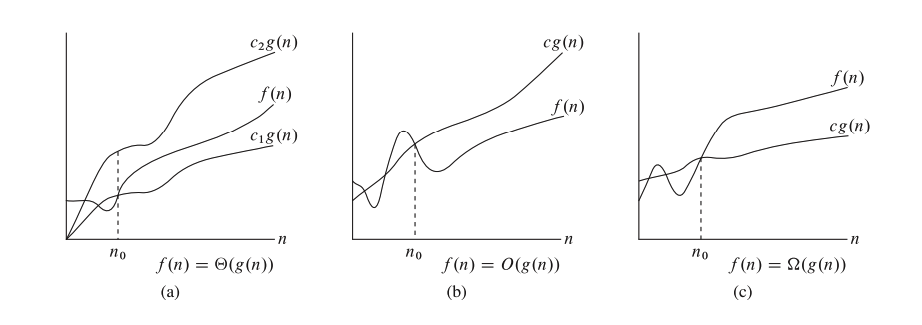
\includegraphics[width=0.85\textwidth]{image1.png}
\end{center}

\textbf{Quick example:} if $f(n) = 3n + 10$, then $f(n) = O(n)$, because for large $n$ it
grows like $n$ (constants don't matter).

\slide{17}{Poll: which sets contain this function?}
\poll{Which of these sets contain $n^2 + n^{4.5} + \sqrt{n} + \log n$? (multiple choice)}

\paragraph{Worked solution.}
We want to know which Big-O / $\Theta$ / $\Omega$ ``sets'' include the function
\[
  f(n) = n^2 + n^{4.5} + \sqrt{n} + \log n.
\]

\textbf{1) Find the dominant term.}
As $n$ gets large, the term that grows fastest dominates everything else. Compare the powers:
\begin{itemize}
  \item $n^{4.5}$ grows faster than $n^2$.
  \item $n^{4.5}$ grows much faster than $\sqrt{n} = n^{0.5}$.
  \item $n^{4.5}$ grows much faster than $\log n$.
\end{itemize}
So for large $n$, $f(n) \approx n^{4.5}$. More formally: $f(n) = \Theta(n^{4.5})$.

\textbf{2) What sets contain it?}
Because $f(n) = \Theta(n^{4.5})$, all of these are true:
\begin{itemize}
  \item \textbf{Big-Theta:} $f(n) \in \Theta(n^{4.5})$.
  \item \textbf{Big-O (upper bounds):} $f(n) \in O(n^{4.5})$, $O(n^5)$, $O(n^{10})$, $O(2^n)$, etc.
        (any function that grows \emph{at least as fast} as $n^{4.5}$ can be an upper bound).
  \item \textbf{Big-Omega (lower bounds):} $f(n) \in \Omega(n^{4.5})$, $\Omega(n^2)$,
        $\Omega(\sqrt{n})$, $\Omega(\log n)$, $\Omega(1)$
        (any function that grows \emph{no faster} than $n^{4.5}$ can be a lower bound).
\end{itemize}

\textbf{3) What it is NOT in:}
\begin{itemize}
  \item Not in $O(n^2)$ (because $n^{4.5}$ eventually dwarfs $n^2$).
  \item Not in $\Theta(n^2)$, $\Theta(n^5)$, etc. (Theta must match the growth rate).
\end{itemize}

\slide{18}{Building math vocabulary: the full family}
\textbf{Big picture:} think of $f(n)$ as the ``real cost'' (time, steps, etc.) and $g(n)$ as
a ``reference growth''. We only care about what happens \textbf{after some point} $n_0$
(when $n$ is big).

\textbf{1) Big-O: $f(n) = O(g(n))$ (upper bound).}
Meaning: $f$ grows \emph{no faster} than $g$ (up to a constant). After $n_0$,
$f(n) \le c \cdot g(n)$ for some constant $c$.
Plain English: ``$g(n)$ is a \emph{ceiling} for $f(n)$ (ignoring constant factors).''
Example: $3n + 10 = O(n)$.

\textbf{2) Big-Omega: $f(n) = \Omega(g(n))$ (lower bound).}
Meaning: $f$ grows \emph{at least as fast} as $g$ (up to a constant). After $n_0$,
$f(n) \ge c \cdot g(n)$.
Plain English: ``$g(n)$ is a \emph{floor} for $f(n)$.''
Example: $3n + 10 = \Omega(n)$.

\textbf{3) Big-Theta: $f(n) = \Theta(g(n))$ (tight bound).}
Meaning: \emph{same growth rate}. It is both $O(g(n))$ (not faster) and $\Omega(g(n))$
(not slower), so $f$ is ``sandwiched'' between two multiples of $g$.
Example: $3n + 10 = \Theta(n)$.
That is why $\Theta(g(n)) = O(g(n)) \cap \Omega(g(n))$ (intersection = both true).

\textbf{4) little-o: $f(n) = o(g(n))$ (strictly smaller).}
Meaning: $f$ grows \emph{slower} than $g$ (not just ``not faster''). In fact, no matter how
small a constant $c$ you pick, eventually $f(n) < c \cdot g(n)$.
Example: $n = o(n^2)$.

\textbf{5) little-omega: $f(n) = \omega(g(n))$ (strictly larger).}
Meaning: $f$ grows \emph{faster} than $g$. No matter how big a constant $c$ you pick,
eventually $f(n) > c \cdot g(n)$.
Example: $n^2 = \omega(n)$.

\textbf{Formal definitions:}
\begin{itemize}
  \item $f(n) = O(g(n)) \iff \exists c > 0,\ n_0$ such that $|f(n)| \le c \cdot g(n)\ \ \forall n \ge n_0$.
  \item $f(n) = \Omega(g(n)) \iff \exists c > 0,\ n_0$ such that $|f(n)| \ge c \cdot g(n)\ \ \forall n \ge n_0$.
  \item $\Theta(g(n)) = O(g(n)) \cap \Omega(g(n))$.
  \item $f(n) = o(g(n)) \iff \forall c > 0,\ \exists n_0$ such that $|f(n)| < c \cdot g(n)\ \ \forall n \ge n_0$. (strictly slower growth)
  \item $f(n) = \omega(g(n)) \iff \forall c > 0,\ \exists n_0$ such that $|f(n)| > c \cdot g(n)\ \ \forall n \ge n_0$. (strictly faster growth)
\end{itemize}

\textbf{Memory shortcut:} O = ``at most'', $\Omega$ = ``at least'', $\Theta$ = ``same'',
$o$ = ``strictly less'', $\omega$ = ``strictly more''.

\slide{19}{Poll: $f(n) = \log^2 n$}
\poll{Select all that apply: $f(n) = \log^2 n$}

\slide{20}{Poll: comprehension check}
\poll{How well do you understand Big-O? (rating)}

\section{Divide and Conquer}

\slide{21}{Back to the Max-Profit problem}
Divide and Conquer approach:
\begin{itemize}
  \item Define subproblems (smaller instances) that can be solved independently.
  \item \textbf{Optimal substructure}: an optimal solution contains optimal solutions to subproblems.
  \item We can build an optimal solution for the original problem using optimal solutions to subproblems.
\end{itemize}
\begin{itemize}
  \item Hard part: defining the subproblems.
\end{itemize}

\slide{22}{Subproblems: split $A$ in half}
Three cases:
\begin{enumerate}
  \item OPT is entirely in the left subproblem: $A[low..mid]$
  \item OPT is entirely in the right subproblem: $A[mid+1..high]$
  \item OPT crosses the midpoint \hfill (pair discussion)
\end{enumerate}
(Diagram: array segment with indices $low$, $mid$, $mid+1$, $high$; cases 1--2 entirely on one side of the split, case 3 crossing the midpoint.)

\slide{23}{Case 3: structure of the crossing OPT}
\begin{itemize}
  \item If an oracle told you OPT crosses the midpoint, what can you say about $A[i]$ and $A[j]$?
  \item Can $A[i]$ be greater than $\min(A[low..mid])$? (No.)
  \item Then OPT is
  \[
    \left( \argmin_{i \in [low..mid]} A[i],\; \argmax_{j \in [mid+1..high]} A[j] \right).
  \]
\end{itemize}
(Small example: days 0--4 with prices $10, 11, 7, 10, 6$.)

\slide{24}{Full example}
Divide and Conquer approach:
\begin{itemize}
  \item Divide subproblems.
  \item Compute solutions to subproblems.
  \item Compute the crossing solution.
  \item Return the best of the 3 cases.
\end{itemize}
(Small example: days 0--4 with prices $10, 11, 7, 10, 6$.)

\slide{25}{Correctness + pseudocode}
Divide and Conquer:
\begin{itemize}
  \item Show optimal substructure:
  \begin{itemize}
    \item Case analysis + contradiction
    \item Induction $\sim$ Recursion
  \end{itemize}
\end{itemize}

\begin{alltt}
\textbf{Max-Profit-D\&C}(\(A, low, high\))
    \textbf{if} \(low == high\)
        \textbf{return} \((low, high)\)
    \textbf{else} \(mid = \lfloor (low + high)/2 \rfloor\)
        \((l_i, l_j) =\) \textbf{Max-Profit-D\&C}(\underline{\hspace{1.5cm}})
        \((r_i, r_j) =\) \textbf{Max-Profit-D\&C}(\underline{\hspace{1.5cm}})
        \((c_i, c_j) = (\) \textbf{Find-min-index}(\underline{\hspace{1.2cm}}), \textbf{Find-max-index}(\underline{\hspace{1.2cm}})\()\)
    \textbf{return} best \((x_i, x_j)\) with \(x \in \{l, r, c\}\)
\end{alltt}

\slide{26}{Time analysis}
Recurrence describing $T(n)$:

\begin{alltt}
\textbf{Max-Profit-D\&C}(\(A, low, high\))
    \textbf{if} \(low == high\)
        \textbf{return} \((low, high)\)
    \textbf{else} \(mid = \lfloor (low + high)/2 \rfloor\)
        \((l_i, l_j) =\) \textbf{Max-Profit-D\&C}(\(A, low, mid\))
        \((r_i, r_j) =\) \textbf{Max-Profit-D\&C}(\(A, mid+1, high\))
        \((c_i, c_j) = (\) \textbf{Find-min-index}(\(A, low, mid\)), \textbf{Find-max-index}(\(A, mid+1, high\))\()\)
    \textbf{return} best \((x_i, x_j)\) with \(x \in \{l, r, c\}\)
\end{alltt}

\paragraph{Plain-English walkthrough (D\&C for Max-Profit).}
The algorithm is a \textbf{Divide-and-Conquer solution for the Max-Profit problem}.

\textbf{1) The Max-Profit problem.} Given prices over days (e.g., $10, 11, 7, 10, 6$ on days
0--4), buy at a low price and sell later at a high price to maximize profit. Example: buy on
day 2 for $7$, sell on day 3 for $10$, profit $= 10 - 7 = 3$. The goal is to find the pair
\texttt{(buy day, sell day)} with the largest positive difference.

\textbf{2) Divide the array in half.} Split around the middle:
\begin{alltt}
         mid
          \(\downarrow\)
[10, 11, 7] | [10, 6]
   LEFT        RIGHT
\end{alltt}
The best solution is in exactly one of three cases:
\begin{itemize}
  \item \textbf{Case 1:} entirely on the left --- find the best buy/sell pair using only the left side.
  \item \textbf{Case 2:} entirely on the right --- find the best pair using only the right side.
  \item \textbf{Case 3:} crosses the middle --- the purchase happens on the \textbf{left}, the sale
        on the \textbf{right}, because the transaction crosses the midpoint.
\end{itemize}

\textbf{3) Finding the crossing solution.} For a crossing solution:
\begin{itemize}
  \item \textbf{Buy side:} take the \emph{minimum} price on the left. Left side $10, 11, 7$:
        minimum $= 7$, so buy $= 7$.
  \item \textbf{Sell side:} take the \emph{maximum} price on the right. Right side $10, 6$:
        maximum $= 10$, so sell $= 10$.
  \item Crossing profit $= 10 - 7 = 3$.
\end{itemize}

\textbf{4) Why minimum on the left and maximum on the right?}
Suppose the optimal crossing solution buys at position $i$ and sells at $j$. If $A[i]$ is not
the smallest value on the left, some $A[k] < A[i]$ exists and we could buy at $k$ instead,
giving at least as much profit. Similarly, if $A[j]$ is not the largest value on the right, we
could sell higher and earn more. Therefore, for a crossing solution: \textbf{buy at the minimum
price on the left and sell at the maximum price on the right}. That is why the algorithm
computes $\min(A[low..mid])$ and $\max(A[mid+1..high])$ and the profit
$\mathit{max\_right} - \mathit{min\_left}$.

\textbf{5) Three answers at every recursive step.}
\begin{alltt}
left  = solve(left half)                  best profit completely in LEFT
right = solve(right half)                 best profit completely in RIGHT
cross = max(right side) - min(left side)  best profit starting LEFT, ending RIGHT

return best of: left, right, cross
\end{alltt}

\textbf{6) What the recursion does.} Keep splitting the array; at a single element there is
nothing to buy and sell within one day, so that is the \textbf{base case}. Then the algorithm
works its way back up, comparing the three possibilities at every level.

\textbf{7) The pseudocode, without the notation.} It is basically:
\begin{quote}
\textbf{Split $\to$ solve left $\to$ solve right $\to$ solve crossing $\to$ pick the best.}
\end{quote}

\textbf{8) Full example.} For prices $10, 11, 7, 10, 6$ (days 0--4) the best transaction is
buy day 2 at \$7, sell day 3 at \$10, profit \$3. The algorithm discovers this by comparing
LEFT, RIGHT, and CROSS at each level and choosing the largest profit.

\textbf{9) Why is this useful?} Brute force compares every buy/sell pair: $O(n^2)$. Divide and
Conquer splits the problem in half and recursively solves it, with recurrence
$T(n) = 2T(n/2) + O(n)$ (the $O(n)$ comes from finding the minimum on the left and the maximum
on the right). By the Master Theorem, $T(n) = O(n \log n)$:
\begin{center}
  Brute force: $O(n^2)$ \qquad vs. \qquad Divide \& Conquer: $O(n \log n)$.
\end{center}

\textbf{The one sentence to memorize:} \emph{Divide the array in half, find the best solution
on the left, the best on the right, and the best solution crossing the middle; then return the
best of the three.} And for the crossing case specifically: \emph{buy at the minimum price on
the left and sell at the maximum price on the right.}

\paragraph{Python implementation.}
\begin{alltt}
def max_profit_dc(A, low, high):
    # Base case: only one day
    if low == high:
        return (low, high)

    # Find the middle
    mid = (low + high) // 2

    # Case 1: best solution entirely in the left half
    left = max_profit_dc(A, low, mid)

    # Case 2: best solution entirely in the right half
    right = max_profit_dc(A, mid + 1, high)

    # Case 3: best solution crosses the midpoint
    min_index = low
    for i in range(low, mid + 1):
        if A[i] < A[min_index]:
            min_index = i

    max_index = mid + 1
    for j in range(mid + 1, high + 1):
        if A[j] > A[max_index]:
            max_index = j

    cross = (min_index, max_index)

    # Choose the best of the three
    left_profit = A[left[1]] - A[left[0]]
    right_profit = A[right[1]] - A[right[0]]
    cross_profit = A[cross[1]] - A[cross[0]]

    if left_profit >= right_profit and left_profit >= cross_profit:
        return left
    elif right_profit >= left_profit and right_profit >= cross_profit:
        return right
    else:
        return cross
\end{alltt}

\slide{27}{Poll: solving the recurrence}
\poll{What is the solution of the recurrence? (multiple choice)}

\paragraph{Worked solution.}
You have a \textbf{recurrence} that describes how long an algorithm takes:
\[
  T(n) = 2 \cdot T(n/2) + \Theta(n)
\]
\begin{itemize}
  \item $T(n)$ = time for input size $n$.
  \item $2 \cdot T(n/2)$ = we solve 2 smaller problems, each half the size.
  \item $+\ \Theta(n)$ = extra work to combine results (like merging).
\end{itemize}

\textbf{What is the solution?}
If you \emph{expand} this pattern:
\begin{itemize}
  \item Level 0: work $= \Theta(n)$.
  \item Level 1: 2 problems of size $n/2$, work $= 2 \cdot \Theta(n/2) = \Theta(n)$.
  \item Level 2: 4 problems of size $n/4$, work $= 4 \cdot \Theta(n/4) = \Theta(n)$.
\end{itemize}
Each \textbf{level} does $\Theta(n)$ work. How many levels? You keep dividing $n$ by 2 until
you reach 1, so that is $\log_2 n$ levels.
\[
  \text{Total work} = \Theta(n) \cdot \log_2 n = \Theta(n \log n).
\]

\textbf{Two methods to find this:}
\begin{itemize}
  \item \textbf{Recursion tree:} draw the tree of recursive calls; notice each level costs
        $\Theta(n)$; count levels $\to \log n$; gives the answer $\Theta(n \log n)$.
  \item \textbf{Substitution method:} \emph{guess} the answer (use the recursion tree to
        guess), then \emph{prove} it with induction (like a math proof). In this course, a
        super formal proof is not required.
\end{itemize}

\textbf{Final simple answer:}
\[
  T(n) = \Theta(n \log n) \quad \text{(like Merge Sort).}
\]
That's it --- you split in half, do linear work at each level, and there are $\log n$ levels.

\section{Solving Recurrences}

\slide{28}{Recursion tree method}
\[
  T(n) \le
  \begin{cases}
    \Theta(1) & \text{if } n = 1,\\[0.5ex]
    2 \cdot T(n/2) + \Theta(n) & \text{otherwise.}
  \end{cases}
\]
\begin{itemize}
  \item Relies on noticing a pattern.
  \item For a formal proof, one must show that the pattern holds for all levels.
  \item We will not be very formal with this method in this course.
\end{itemize}

\slide{29}{Substitution method}
\begin{itemize}
  \item Basically, induction using the definition of Big-O/Omega.
  \item We need to guess the answer (use the recursion tree first, for example).
\end{itemize}
\[
  T(n) = 2 \cdot T(n/2) + \Theta(n)
\]

\paragraph{Detailed walkthrough: recursion tree and substitution.}

\textbf{1) What does the recurrence mean?}
Think of it as: a \textbf{problem of size $n$} is split into \textbf{2 smaller problems}, each
of size $n/2$, and we spend $\Theta(n)$ extra work to combine them:
\begin{alltt}
                 T(n)
               /      \
           T(n/2)    T(n/2)
           /  \       /  \
        T(n/4) ...  ...  T(n/4)
\end{alltt}
Three important pieces: \textbf{2} = number of subproblems, \textbf{$n/2$} = size of each
subproblem, \textbf{$\Theta(n)$} = work done outside the recursive calls.

\textbf{2) Recursion tree method.}
The idea: \emph{draw the tree and add up the work at each level.}
\begin{itemize}
  \item \textbf{Level 0:} 1 problem: $\Theta(n)$.
  \item \textbf{Level 1:} 2 problems, each doing $\Theta(n/2)$:
        total $2 \cdot \Theta(n/2) = \Theta(n)$.
  \item \textbf{Level 2:} 4 problems, each doing $\Theta(n/4)$:
        total $4 \cdot \Theta(n/4) = \Theta(n)$.
\end{itemize}
\begin{alltt}
Level 0:        \(\Theta(n)\)
                 |
Level 1:     \(\Theta(n/2) + \Theta(n/2) = \Theta(n)\)
              /          \
Level 2:   4 \(\times\) \(\Theta(n/4) = \Theta(n)\)
                 ...
\end{alltt}
\emph{Every level costs $\Theta(n)$.}

\emph{How many levels?} Every time we divide $n$ by 2,
$n \to n/2 \to n/4 \to n/8 \to \cdots$, and we stop when we reach 1:
\[
  \frac{n}{2^k} = 1 \quad\Longrightarrow\quad 2^k = n \quad\Longrightarrow\quad k = \log_2 n.
\]
So there are approximately $\log n$ levels. Since each level costs $\Theta(n)$:
\[
  T(n) = \Theta(n) \times \Theta(\log n)
  \qquad\Longrightarrow\qquad
  \boxed{T(n) = \Theta(n \log n)}.
\]
\textbf{Recursion tree shortcut:} if \emph{each level has the same cost} and there are
$\log n$ levels, the answer is $n \log n$.

\textbf{3) Substitution method.}
The slide says: ``basically, induction using the definition of Big-O/Omega.'' The idea:
\emph{guess the answer first, then prove that your guess is correct.}
From the recursion tree we already guessed $T(n) = \Theta(n \log n)$. Now we prove it.
Suppose $T(n) \le c\, n \log n$ for some constant $c$. Substitute this into the recurrence
(ignoring constants for simplicity):
\[
  T(n) \le 2\left[ c\,\frac{n}{2} \log\frac{n}{2} \right] + cn
        = cn(\log n - 1) + cn
        = cn\log n - cn + cn
        = cn\log n.
\]
So our guess works, giving $T(n) = O(n \log n)$. You similarly prove the lower bound
$T(n) = \Omega(n \log n)$, and therefore
\[
  \boxed{T(n) = \Theta(n \log n)}.
\]
\textbf{Easy way to remember substitution:} \emph{Guess $\to$ Substitute $\to$ Prove.}

\slide{30}{Master method (theorem) recap}
\[
  T(n) = a \cdot T(n/b) + f(n)
\]
Idea: compare $f(n)$ (root level) with $n^{\log_b a}$ (leaf level).
\begin{itemize}
  \item \textbf{Case 1:} $f(n) = O(n^{(\log_b a) - \epsilon})$ \hfill (polynomially smaller; leaf level dominates)
        \[ T(n) = \Theta(n^{\log_b a}) \]
  \item \textbf{Case 2:} $f(n) = \Theta(n^{\log_b a})$ \hfill (all levels about the same)
        \[ T(n) = \Theta(n^{\log_b a} \log n) \]
  \item \textbf{Case 3:} $f(n) = \Omega(n^{(\log_b a) + \epsilon})$, and \ldots \hfill (root level dominates)
        \[ T(n) = \Theta(f(n)) \]
\end{itemize}

\paragraph{Detailed explanation.}
The Master Theorem is a quick way to solve running times of divide-and-conquer algorithms that
look like
\[
  T(n) = a\,T\!\left(\frac{n}{b}\right) + f(n).
\]

\textbf{What the parts mean:}
\begin{itemize}
  \item $a$: how many subproblems you create.
  \item $n/b$: each subproblem size (you shrink the input by factor $b$).
  \item $f(n)$: extra work you do outside the recursive calls (splitting, merging, etc.).
\end{itemize}

\textbf{The key comparison.} Compute this ``benchmark'':
\[
  n^{\log_b a}
\]
This represents the total work at the \textbf{bottom (leaves)} of the recursion tree. Then
compare $f(n)$ to $n^{\log_b a}$. Three cases:

\textbf{Case 1: $f(n)$ is smaller (leaves dominate).}
If
\[
  f(n) = O\!\left(n^{\log_b a - \epsilon}\right)
\]
(meaning $f(n)$ is polynomially smaller), then
\[
  T(n) = \Theta\!\left(n^{\log_b a}\right).
\]
\emph{Simple idea:} most cost comes from doing many small subproblems.

\textbf{Case 2: $f(n)$ is about the same size (all levels add up).}
If
\[
  f(n) = \Theta\!\left(n^{\log_b a}\right),
\]
then
\[
  T(n) = \Theta\!\left(n^{\log_b a} \log n\right).
\]
\emph{Simple idea:} each level of recursion costs about the same, and there are $\log n$ levels.

\textbf{Case 3: $f(n)$ is bigger (top/root dominates).}
If
\[
  f(n) = \Omega\!\left(n^{\log_b a + \epsilon}\right)
\]
(and it satisfies a ``regularity condition'', basically meaning it stays bigger consistently),
then
\[
  T(n) = \Theta(f(n)).
\]
\emph{Simple idea:} the extra work $f(n)$ at the top overwhelms everything else.

\textbf{Tiny examples:}
\begin{itemize}
  \item \emph{Merge sort:} $T(n) = 2T(n/2) + n$. Here $n^{\log_2 2} = n$, which matches
        $f(n) = n$ $\Rightarrow$ Case 2 $\Rightarrow$ $T(n) = \Theta(n \log n)$.
  \item \emph{Binary search:} $T(n) = T(n/2) + 1$. Here $n^{\log_2 1} = 1$, which matches
        $f(n) = 1$ $\Rightarrow$ Case 2 $\Rightarrow$ $T(n) = \Theta(\log n)$.
\end{itemize}

\slide{31}{Poll: practice with the master method}
\poll{Solve the recurrence $T(n) = 4 \cdot T(n/2) + n \log n$. (multiple choice)}

\section{Summary}

\slide{32}{Review}
(Small example: prices $10, 11, 7, 10, 6$ over days 0--4, with the divide-and-conquer split diagram.)
\begin{itemize}
  \item Brute force: $O(n^2)$-time algorithm.
  \item Divide and Conquer: $O(n \log n)$-time algorithm.
  \item Next: Dynamic programming --- ``smarter'' D\&C: dealing with subproblems better.
  \item Typically: optimal substructure + overlapping subproblems.
\end{itemize}

\end{document}
